\documentclass[%
	pdftex,
	oneside,        % One-sided print
	11pt,           % Font size
	parskip=half,   % The half of a line margin after line feeds
	headsepline,    % Line after header
	footsepline,    % Line after footer
	abstracton,     % Abstract headings
	USenglish,      % Written in English
	a4paper,        % Written on Din A4 paper
]{report}


\title{Knowledge based systems\\ Analysing the eligibility of a person for higher education using a Bayesian network}
\author{Lisa Mischer \& Frank Steiler\\ Interactive and knowledge based systems (T2INF4307)\\ DHBW Stuttgart\\ Contact: it12147@lehre.dhbw-stuttgart.de\\\\ \url{http://www.github.com/steilerDev/WhatToStudy}}
        
\usepackage[english]{babel}
\usepackage[english=british]{csquotes}
\usepackage[style=alphabetic,backend=biber,natbib=true]{biblatex}
\addbibresource{Documentation.bib}
\usepackage{graphicx}
\usepackage{setspace}
\usepackage{hyperref}
\usepackage{varioref}
\usepackage{chngcntr}
\usepackage{subcaption}
\usepackage[export]{adjustbox}[2011/08/13]
\usepackage{fancyhdr}
\usepackage[toc,page]{appendix}
\usepackage{pdfpages}
\usepackage{tabularx}
\usepackage{longtable}
\usepackage{float}
\usepackage{pifont}
\usepackage{rotating}
\usepackage{pdflscape}

\usepackage{color}
\definecolor{ListingBackground}{rgb}{0.92,0.92,0.92}

\usepackage{listings}
\lstset{
    basicstyle=\normalfont\ttfamily,
    language=java,
    extendedchars=true,
    backgroundcolor=\color{ListingBackground},
    frame=single,
    numbers=left,
    tabsize=8,
    numberstyle=\scriptsize,
    stepnumber=1,
    numbersep=8pt,
    keepspaces=true, 
    breaklines=true,
    showstringspaces=false
}

\hypersetup{
	colorlinks=true,
    citecolor=black,
    filecolor=black,
    linkcolor=black,
    urlcolor=black,
	pdftitle=Analysing the eligibility of a person for higher education using a Bayesian network,
	pdfauthor={Lisa Mischer \& Frank Steiler}, 
	pdfcreator={Lisa Mischer \& Frank Steiler},
	pdfproducer={Lisa Mischer \& Frank Steiler},
	pdfdisplaydoctitle=true
}

\restylefloat{table}

\onehalfspacing


\pagestyle{fancy}
\lhead{}
\renewcommand{\headrulewidth}{0pt}
\setlength{\headheight}{14pt}

\newcommand{\nocontentsline}[3]{}
\newcommand{\tocless}[2]{\bgroup\let\addcontentsline=\nocontentsline#1{#2}\egroup}

\begin{document}

\counterwithout{figure}{chapter}
\counterwithout{table}{chapter}
\counterwithout{lstlisting}{chapter}
\counterwithout{equation}{chapter}

\newcounter{magicrownumbers}[table]

\maketitle

\newpage
\thispagestyle{empty}
\mbox{}
\setcounter{page}{0}

\tableofcontents

\chapter{Introduction}
Within knowledge based systems, logic is a commonly used way to represent connections between data and expressions. Unfortunately logic can not handle uncertainty or imprecise data. Bayesian Networks have been developed to tackle this problem, by representing knowledge as a set of variables and their dependencies within a directed acyclic graph. \cite{Reichardt:2014aa}

A probabilistic network is using conditional probabilities between the nodes of the graph and inferences to calculate the probability of symptoms and/or causes. There are three types of inferences that are occurring in the network and enable the functionality of the graph: diagnostic, causal and inter-causal inference.

A Bayesian Network is defined by a set of edges (nodes) connected through vertices within a graph: $D=(V,E)$. Every node has finite set of mutually exclusive states. On top of that the network is quantifying the dependencies within a separated conditional probability table (CPT) for each node. \cite{Vomlel:2005aa}

Concluding to create and then use a Bayesian Network, a user has to create the correct graph first and then determine all values for the CPT. A correct network can either be created by an expert, by using data mining techniques to find connections between entities and machine learning to specify the CPT values. 

By adding observations for a specific case to the network, it is updating beliefs about other variables. Furthermore the probability of a certain event or state can be predicted by observing other events or states. Therefore it can support decision making and has numerous applications, like the diagnosis of diseases, automatic troubleshooting or education testing. \cite{Vomlel:2005aa}

\chapter{Preparation of data}
As part of our exercise we received a set of data that was supposed to help us derive the structure of the network. To be able to use the stated cases we first had to analyse and harmonise the provided data. 

These preparation included the transformation of continuous variables into discrete ones, to enable their usage within the network. The variables we had to adjust were all provided grades, the test results of the online tests and study ability test, as well as the parental income. 

Furthermore we chose a general syntax for the naming of values, to have standardised identifiers and consistent ranges. E.g. we defined a not available value as "NA", where the source used different words in different entities, like "keine", "n.a." and many more. We did not need to do this necessarily, but it simplified the work with the network.

A detailed description about the conversation of these values can be found within the documentation of the implementation in chapter \vref{chapter:WhatToStudy}, more specific in section \vref{sec:CaseFile}.

These preparations were necessary to train the Bayesian network, as well as to analyse a certain case. Only cases which are prepared in the same way can be evaluated with our result network, but the implementation is able to read a cleaned

\chapter{Structure of the network}
To find the best structure of the network, we took a look at the provided information, trying to find connections between columns of the data set. 

Therefore we plotted the data within a parallel coordinate system, shown in appendix \vref{app:Parallel}. We used this representation to derive connections by reducing the data on a single axis to a smaller range and hoping to observe a similar behaviour on another axis. By revealing such a influence we concluded a direct connection between the entities.

On top of that we thought about logical connections, e.g. the mathematics', German's and physic's grade had to influence the qualification average. Furthermore, we took it for granted that the mathematics grade influences the results of the math online test, as well as the German grade influences the results of the German online test. Moreover the mathematics results influence the physics grade, since a basic understanding of mathematics is essential for physics. 

To determine whether or not our Bayesian network is suited to predict the final grade of a specific student, we tested it using the provided data set. This test tried to predict the final grade of a person, using all available information from the data excluding the actual course and the actual final grade. By comparing the predicted and the actual result, we received an error rate for our network. We used this error rate to compare different versions of the network.

The generation of the final network was an iterative process, changing the arcs, CPTs and/or entities within each step. After changing the structure, we determined the new error rate and compared it to the previous one. By using this process we were able to improve the overall performance of the network. In the end, all our considerations at the beginning proved as wrong, since there is no indirect influence on a variable, only direct.

We were able to achieved an error rate of 11\%, predicting the course taken, and 4\%, predicting the final grade of a student. Appendix \vref{app:Network} is showing our final Bayesian network. The implementation documented in chapter \vref{chapter:WhatToStudy} is using a slightly different Network, since the optimal one is too big, resulting in a out of memory error of the Java virtual machine. In the adjusted net the gender of a person is no longer considered, to reduce its size. Nevertheless, the error rate only rises slightly to 14\%, respectively 6\%. This network is then used to recommend for or against studying a specific course. 

The tool we used to specify our Bayesian network is called Netica, unfortunately we only had access to a limited version of this program. Concluding, it was necessary to limit our data set to 15 entities. Therefore we had to leave out at least one piece of information and take a slightly more imprecise result into account. We chose to ignore the information about the state, even though it improved the error rate significantly, when taking only 5 of 16 states into account. Unfortunately it is necessary to accept all 16 available states, since all of them could be chosen. This resulted in an entity with 16 different parameter values, which were too much to handle for Netica. Since it was not reasonable to allow only 5 parameter values, we decided to leave this entity out of consideration. Furthermore we left out the income of the parents and the nationality, since these did not provide any gain in information to the network.

\chapter{Learning conditional probability tables}
\label{chapter:Learning}
After creating a draft of the network layout, containing all plausible node connections, we had to quantify the dependencies between nodes within the conditional probability tables (CPT). Since we were not able to consult an expert about this problem we chose to use machine learning algorithms to generate the tables.

Fortunately the tool we used to specify the network offered a set of machine learning algorithms to generate the CPTs from a data set. These include a \enquote{counting algorithm}, an \enquote{expectation-maximization (EM) algorithm} and a \enquote{gradient descent algorithm}. According to the documentation of the tool the \enquote{counting algorithm} is the simplest and fastest. This algorithm is especially well performing when having no uncertainty or missing data. Concluding if the data set has missing values, the user should either choose the \enquote{EM-algorithm} or the \enquote{gradient descent algorithm}. The performance of either is highly depending on the data set and network structure. Therefore the selection of one algorithm over the other needs to be done by directly comparing their performance. \cite[p. 47]{Corp.:2010aa} 

After comparing the performance of each algorithm using our set of data, we chose to use the \enquote{expectation-maximization (EM) algorithm}, since it fitted our needs best. \enquote{Briefly, Expectation Maximization learning repeatedly takes a Bayes net and uses it to find a better one by doing an expectation step followed by a maximization step. In the expectation step, it uses regular Bayes net inference with the existing Bayes net to compute the expected value of all the missing data, and then the maximization step finds the maximum likelihood Bayes net given the now extended data.} \cite[p. 48]{Corp.:2010aa}

After applying the algorithm with several hundert iterations using the provided data set we could create a network that reliably predicted the final grade and therefore could give a recommendation based on all provided values. As mentioned earlier the error rate at predicting the final grade correctly is 4\%. Testing the quality of the network based on the correct recommendation of studying the selected course and using the worse network mentioned in chapter \vref{chapter:Learning}, achieves an error rate of 2\%, where no error is false positive (Recommending the course even if the student is probably not going to succeed). This testing is done within the application and its precise documentation can be found in section \vref{sec:Test}.

\chapter{Implementation - WhatToStudy}
\label{chapter:WhatToStudy}
As part of the project a program had to be implemented that is using a Bayesian network and user specific input to give a recommendation for or against studying a specific course. This program was implemented using Java 8 and the NeticaJ library. 

Within this chapter the general functionality and usage of the program is going to be described. For a in-depth documentation of the complete application see the JavaDoc webpage, bundled with this document, or the source code of the application, which is licensed using a GNU General Public License version 2. The complete project and all used assets are hosted on Github (\url{http://www.github.com/steilerDev/WhatToStudy}).

\section{General usage}
The easiest way to start the application is to use the provided \texttt{./run.sh} script. Make sure, that the stated location of the NeticaJ binaries within the script is correct. The NeticaJ binary files can be retrieved from the following URL: \url{https://www.norsys.com/netica-j.html}. 

This project is packed and optimised to run on Macintosh OSX of any version, but since Java is allowing multi platform execution, the start script only needs to be adjusted to your operating system and the correct version of the NeticaJ library needs to be retrieved.

When starting the application without any additional command line arguments you are entering the interactive mode described in section \vref{sec:Interactive}. By adding additional arguments to the program call (or the script execution) you can switch to other modes. A full list of all available modes is given in section \vref{chapter:Modes}, as well as printed to screen when entering the help mode through passing the \texttt{-h} argument (See section \vref{sec:Help}).

\section{Operation modes}
\label{chapter:Modes}
Within this section every available functionality is listed and its functional principles are described.

\subsection{Interactive mode}
\label{sec:Interactive}
When starting the application without any arguments, the user is entering the interactive mode. This mode is requesting personal information one after the other, providing a list of accepted answers. The application is trying to match the user given input with the list of allowed ones until it is accepted.

If the user does not want to give a specific answer, he can always pass an empty String (by hitting the return key without any input). This will most likely lead to a more imprecise prediction than it would be with a complete set of data.

This mode's main task is to collect and parse the user data. After the application gathered the data, it is actually starting to instantiate the evaluation mode, passing the created set of data. The evaluation mode's functionality is described in section \vref{sec:Evaluation}.

\subsection{Evaluation mode}
\label{sec:Evaluation}
Evaluation mode can be entered by passing the \texttt{-e} command line argument together with a case file to the program. The file should be semi-colon separated, with a valid header and only valid values. The exact specification of the input file is given in section \vref{sec:CaseFile}. In contrast to the specification the file does not need to have a value for the final grade or course. The case file is read by the program and only the first case is evaluated, even if it is stating more.

\begin{figure}
    \[ beliefOf(FinalGrade.VeryGood) + \frac{2}{3} \times beliefOf(FinalGrade.Good) \]
    \caption{The used recommendation-rate formula}
    \label{equ:EvaluationFormula}
\end{figure}

\begin{figure}
    \[ beliefOf(FinalGrade.VeryGood) + beliefOf(FinalGrade.Good) \]
    \caption{The conservative recommendation-rate formula}
    \label{equ:ConservativeEvaluationFormula}
\end{figure}

If the student's course is stated within the file, the program is going to evaluate the recommendation rate using the formula shown in figure \ref{equ:EvaluationFormula}. This evaluation was chosen based on testing experience using the provided data and the test mode described in section \vref{sec:Test}. By using this formula the general error rate of a wrong prediction is at 2\% and therefore double as high as choosing the conservative formula shown in figure \vref{equ:ConservativeEvaluationFormula}, but its non-acceptable error rate is 0\% and therefore performs better than the conservative formula.

A non-acceptable error is a false negative error, saying the program is recommending the user to study the course, even if the user is, based on the experience of the network, not going to succeed. Concluding an acceptable error is a false positive one, where the program is discouraging a student to attend the course, even if he would succeed. Since we really did not want to give false negative prediction we were trying to reduce the amount of this kind of error, even if we therefore have to take a slightly higher overall error rate into account.

If the case within the file is not stating the course the student wants to attend, the evaluation is checking the likeliness of a recommendation of every available course by entering the appropriate state within the network and then returning the course with the highest recommendation rate. That means that the program is recommending the course, where the student is most likely going to get a very good or good grade.

Optionally the user can specify a bayesian network, other than the one packaged with the application to evaluate a case. To do so he can pass the path to the network file as a third, optional argument. The file path needs to not contain any white spaces, since those can't be handled by the Java command line interface.

\subsection{Draw mode}
The draw mode can be entered by passing the \texttt{-d} argument to the application during startup. This mode is creating a graphical Java swing frame, which is showing the internally stored Bayesian network. The probabilities of every entity value is displayed as well.

Optionally the user can specify a bayesian network, other than the one packaged with the application to be drawn. To do so he can pass the path to the network file as a second, optional argument. The file path needs to not contain any white spaces, since those can't be handled by the Java command line interface.

\subsection{Learning mode}
A user can enter the learning mode by passing the \texttt{-l} argument as well as the path to a case file (which should not contain any white spaces). The file needs to meet the requirements stated within section \vref{sec:CaseFile}. This mode is using the provided data set to learn the values for the conditional probability tables (CPT) of the network.

Before starting the learning process, every stored value within the CPTs is removed, to avoid unsuitable inference. The used learning algorithm is the \enquote{expectation-maximization (EM) algorithm}. The reason of choosing this algorithm over the other available ones is given in chapter \vref{chapter:Learning}.

After the learning process is finished, the application is writing a file called \enquote{Learned.dne} into the current working directory, overwriting any equally named file. This file is containing all necessary specification for the network as well as the learned CPTs.

Optionally the user can specify a bayesian network, other than the one packaged with the application, whose CPTs should be learned. To do so he can pass the path to the network file as a third, optional argument. The file path needs to not contain any white spaces, since those can't be handled by the Java command line interface.

\subsection{Testing mode}
\label{sec:Test}
To enter the testing mode the user needs to pass the \texttt{-t} argument together with the whitespace-free path to a case file. The cases in the file need to meet the stated requirements for the input files, described in section \vref{sec:CaseFile}.

The test is taking every case, including the information about the course, excluding the final grade, to evaluate the recommendation rate, giving either a recommendation for or against the choice. This recommendation is then compared with the real outcome of the case.

No error occurs, if the program is recommending the student to study the course and he actually achieved a good or very good grade, which would be a true positive prediction. Another correct prediction would be, if the program is discouraging the student to study the selected course and he actually failed or only achieved a satisfying grade, which would be a true negative prediction.

A false positive recommendation is given, if the program discourages the student to study the course, even if he actually achieved a very good or good grade. Concluding the program is giving a false negative prediction if he encourages the student to study the course even if actually failed or only achieved a satisfying grade. A false negative prediction, in contrast to a false positive one, is seen as a non-acceptable error, because we really do not want to encourage a person to waste his time by studying a course he is most likely going to fail. This kind of error should therefore been prevented by all means, even if this means that the overall amount of error is increasing.

At the end of the testing process the program prints out a table containing the result of the test, aggregate into the four categories described in the previous paragraphs. On top of that it provides the error rate (amount of errors over the amount of tests) and the non-acceptable error rate (amount of non-acceptable error over the amount of tests). In an optimal network both rates are as low as possible, but the network should at least be designed in a way to keep the non-acceptable error rate as small as possible.

Optionally the user can specify a bayesian network, other than the one packaged with the application, whose quality should be tested. To do so he can pass the path to the network file as a third, optional argument. The file path needs to not contain any white spaces, since those can't be handled by the Java command line interface.

\subsection{Help mode}
\label{sec:Help}
To enter the help mode the user needs to either pass the \texttt{-h} command line argument or any non-valid argument. This mode is printing out a summary of the general usage of the program, as well as the specification of an input file. This specification is also shown in section \vref{sec:CaseFile}.

\subsection{Version mode}
The version mode is entered by passing the \texttt{-v} argument to the program. This mode is printing out the version number of the application, as well as a list of person involved at creating the application, further acknowledgements, a link to the Github repository of the application and the licensing notice.

\section{Case file handling}
\label{sec:CaseFile}

%Include source code from file using:
%\lstinputlisting[caption=Expected output for the program (implemented using the Bridge design pattern)]{./Source/de/steilerdev/swe/Bridge/output}

%\lstlistoflistings
\printbibliography

\begin{appendices}
%Include pdf for appendix:
    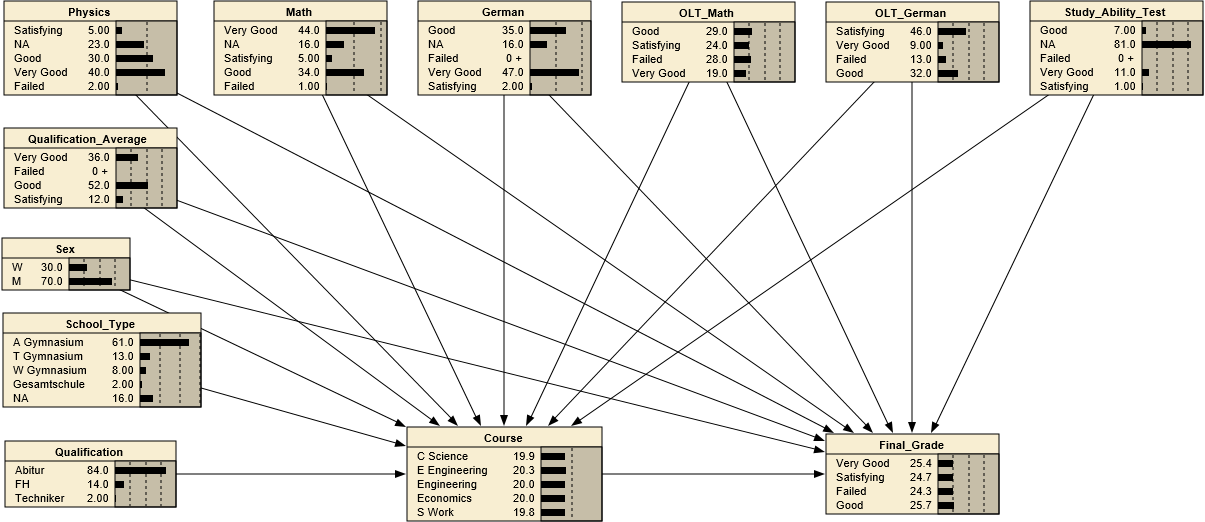
\includepdf[landscape=true,pages=-,addtotoc={1,chapter,0,Bayesian Network,app:Network}]{./assets/StudyNet_Optimal.png}
    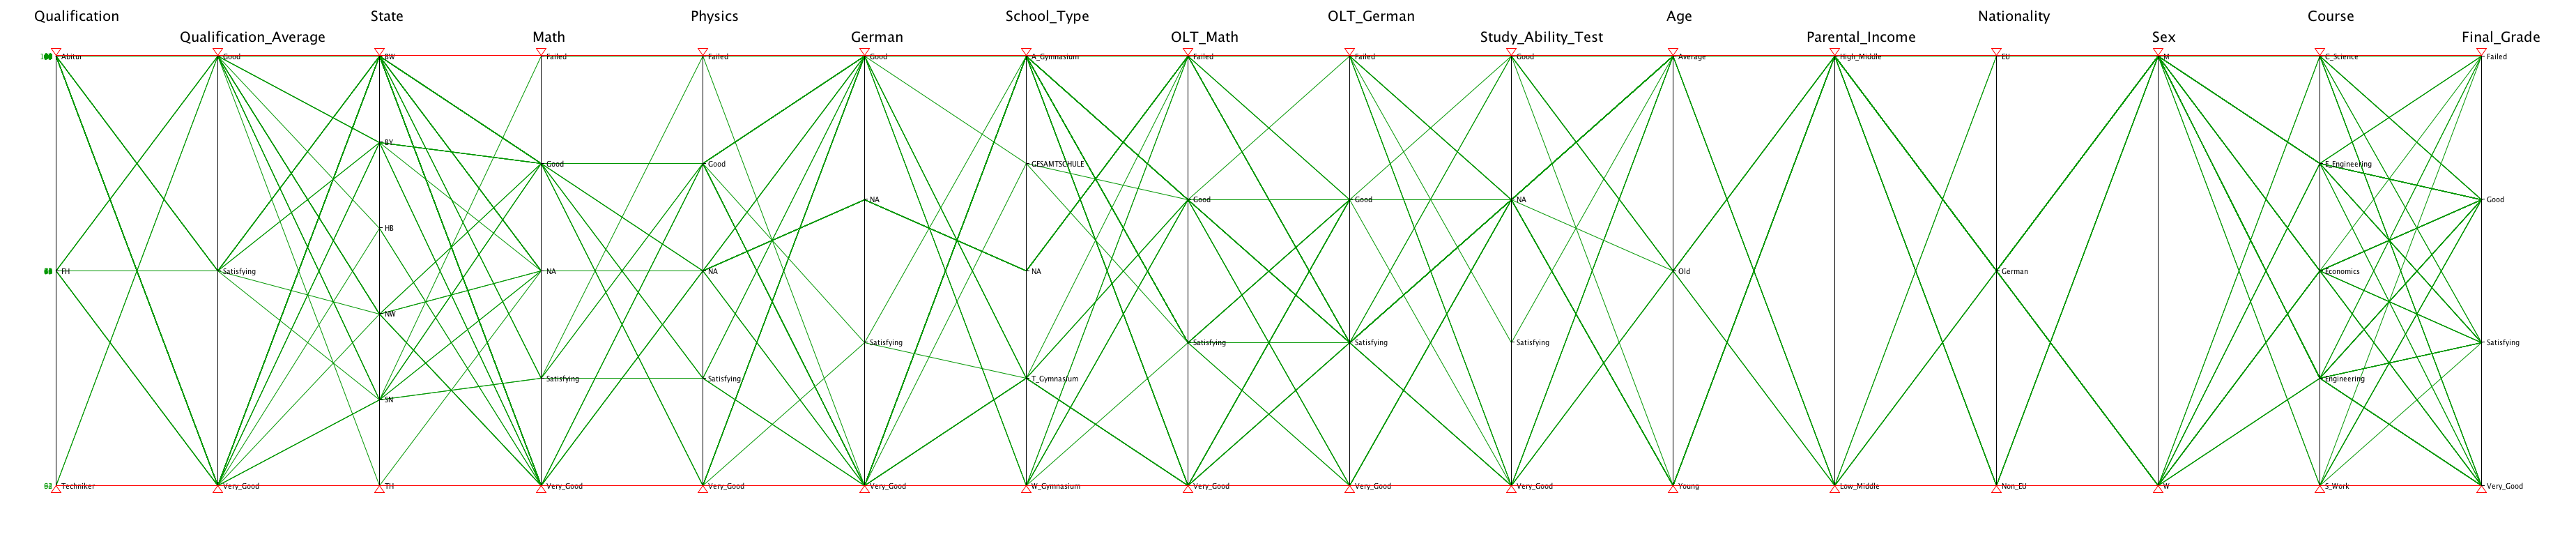
\includepdf[landscape=true,pages=-,addtotoc={1,chapter,0,Data set represented by parallel coordinates,app:Parallel}]{./assets/Parallel.png}
\end{appendices}

\end{document}